\chapter[tNGS can replace Sanger sequencing in clinical diagnostics]{Targeted next-generation sequencing can replace Sanger sequencing in clinical diagnostics}
\chaptermark{targeted NGS in clinical diagnostics}
\label{chap:SNP and Indel detection}

{ \Large \leftwatermark{
		\put(-67,-66.5){ 1 }
		\put(-76.5,-100){
\includegraphics[scale=0.8]{img/thumbindex.eps}} \put(-67,-91.5){ {\color{white} 2 }}
		\put(-67,-116.5){ 3 }
		\put(-67,-141.5){ 4 }
		\put(-67,-166.5){ 5 }
		\put(-67,-191.5){ 6 }
		\put(-67,-216.5){ 7 }
		\put(-67,-241.5){ 8 }
		\put(-67,-266.5){ 9 }
		\put(-67,-291.5){ 10 }
		\put(-67,-316.5){ 11 }
	} \rightwatermark{
		\put(350.5,-66.5){ 1 }
		\put(346.5,-100){
\includegraphics[scale=0.8]{img/thumbindex.eps}} \put(350.5,-91.5){ {\color{white} 2 }}
		\put(350.5,-116.5){ 3 }
		\put(350.5,-141.5){ 4 }
		\put(350.5,-166.5){ 5 }
		\put(350.5,-191.5){ 6 }
		\put(350.5,-216.5){ 7 }
		\put(350.5,-241.5){ 8 }
		\put(350.5,-266.5){ 9 }
		\put(350.5,-291.5){ 10 }
		\put(350.5,-316.5){ 11 }
}}

\hfill \underline{Human Mutation} 2013;34(7):1035-42.

\hfill DOI: \href{https://doi.org/10.1002/humu.22332}{10.1002/humu.22332}

\hfill PubMed ID: \href{https://www.ncbi.nlm.nih.gov/pubmed/23568810}{23568810}

\newpage

\noindent
B. Sikkema-Raddatz\textsuperscript{1}, L.F. Johansson\textsuperscript{1}, E.N. de Boer\textsuperscript{1}, R. Almomani\textsuperscript{1}, L.G. Boven\textsuperscript{1}, M.P. van den Berg\textsuperscript{2}, K.Y. van Spaendonck-Zwarts\textsuperscript{1}, J.P. van Tintelen\textsuperscript{1}, R.H. Sijmons\textsuperscript{1}, J.D.H. Jongbloed\textsuperscript{1},  R.J. Sinke\textsuperscript{1} \\

\noindent
1. University of Groningen, University Medical Center Groningen, Department of Genetics, Groningen, The Netherlands\\
2. University of Groningen, University Medical Center Groningen, Department of Cardiology, Groningen, The Netherlands\\


\noindent
Received 2013 Jan 9; Accepted revised manuscript 2013 Apr 2; Published online 2013 Apr 4.
\\~\\


\section*{Abstract}\label{abstract}
Mutation detection through exome sequencing allows simultaneous analysis of all coding sequences of genes. 
However, it cannot yet replace Sanger sequencing (SS) in diagnostics because of incomplete representation and coverage of exons leading to missing clinically relevant mutations. 
Targeted next-generation sequencing (NGS), in which a selected fraction of genes is sequenced, may circumvent these shortcomings. 
We aimed to determine whether the sensitivity and specificity of targeted NGS is equal to those of SS. 
We constructed a targeted enrichment kit that includes 48 genes associated with hereditary cardiomyopathies. 
In total, 84 individuals with cardiomyopathies were sequenced using 151 bp paired-end reads on an Illumina MiSeq sequencer. 
The reproducibility was tested by repeating the entire procedure for five patients. 
The coverage of $\geq$30 reads per nucleotide, our major quality criterion, was 99\% and in total {\textapprox}21,000 variants were identified. 
Confirmation with SS was performed for 168 variants (155 substitutions, 13 indels). 
All were confirmed, including a deletion of 18 bp and an insertion of 6 bp. 
The reproducibility was nearly 100\%. 
We demonstrate that targeted NGS of a disease-specific subset of genes is equal to the quality of SS and it can therefore be reliably implemented as a stand-alone diagnostic test.

\section{Introduction}\label{introduction}
Next-generation sequencing (NGS) techniques have significantly increased the possibilities of genome analysis. 
If we focus on diagnostic applications, mutation analysis through exome sequencing (ES) allows for the simultaneous analysis of all coding sequences of genes. 
One of the first clinical applications of ES was the detection of disease-associated mutations in rare Mendelian diseases, such as Miller syndrome \cite{Ng_2009}, Sensenbrenner syndrome \cite{Gilissen_2010}, and Schinzel–Giedion syndrome \cite{Hoischen_2010}. 
The advantage of ES is that it does not require a priori knowledge of gene(s) responsible for a disorder using it as a genetic discovery panel. 
In diagnostics, ES is already used to screen for de novo pathogenic mutations in intellectual disability \cite{de_Ligt_2012} explained by more than 1,000 different genes. 
In addition, ES can be used more targeted by analyzing only a panel of genes that may be involved in a particular disease. 

However, in routine diagnostics, detecting mutations via conventional Sanger sequencing (SS) is still the standard, despite the practical difficulties of keeping up with the ever-increasing numbers of test requests and of disease-associated genes. 
For instance, hereditary cardiomyopathies can be explained by 40-60 different genes \cite{Jongbloed_2010,Norton_2012} and effective analysis of all these genes by SS in a diagnostic setting is not feasible. 
In practice, it is limited to no more than 10 genes. 
In contrast, ES would allow the simultaneous analysis of all coding genes through enrichment for these coding regions before sequencing. 
However, in its current state, ES cannot be used as a reliable substitute for SS in diagnostics. 
A major shortcoming is incomplete representation and coverage of exons, leading to clinically relevant mutations being missed \cite{Gilissen_2010,Sulonen_2011}. 
Here, amore dedicated targeted enrichment appears to be the method of choice, not only because it allows focusing on the genes relevant for a particular disorder, but also because its highly effective enrichment provides a superior quality of representation and coverage. 
In addition, focusing on only the genes relevant for a particular disorder minimizes the problems associated with unsolicited findings. 
Targeted NGS is faster and cheaper than ES, especially for the analysis of certain distinct disease phenotypes. 

Various enrichment methods have been developed in the last few years, such as solid phase-based microarrays, micro-droplet-based PCR (Rain Dance Technologies, Lexington, MA), amplicon-based or solution phase-based methods such as Sure Select Targeted enrichment and Illumina TruSeq Custom enrichment. 
Different types of platforms have also been developed for high-throughput sequencing. 
Recently, even bench-top instruments have become available, such as Ion Torrent PGM (Life Technologies Ltd, Paisley, UK), 454 GS Roche Junior (Roche Applied Science, Indianapolis, IN), and the Illumina MiSeq (Illumina, SanDiego,CA) \cite{Loman_2012}. 
These are the size of a modern laser printer and offer modest set-up and running costs; they are particularly suited to small projects and allow a fast throughput. 

The aim of our study was to validate targeted NGS for application in clinical diagnostics and to assess its sensitivity and specificity relative to SS. 
We therefore developed a SureSelect targeted enrichment kit (Agilent Technologies, Inc., Santa Clara, CA) for diagnostic testing of patients with hereditary cardiomyopathies. 
Hereditary cardiomyopathies are highly heterogeneous disorders, and include dilated (DCM), hypertrophic (HCM), and arrhythmogenic right ventricular cardiomyopathies (ARVC), which are leading causes of heart failure and sudden death. 
Approximately 30\%–50\% of DCM cases are familial, but with significant genetic and phenotypic heterogeneity \cite{Posafalvi_2012}. 
Particularly for DCM, for which more than 50 cardiomyopathy-related genes have been identified, targeted resequencing would be a much better diagnostic platform than SS. 
The use of a MiSeq bench-top machine would also enable short turn-around times in the laboratory. 
We compared the outcome of our targeted NGS experiments with results from SS, and discuss our findings in the light of validation, clinical laboratory implementation, and quality assessment in general.

\section{Material and methods}

\subsection{Design of the study}
Our study was divided into two parts: a validation phase and an application phase.

(1) Validation phase in which:
\begin{itemize}
	\item sequencing quality of the targeted NGS kit was measured in terms of representation and coverage;
	\item sequencing reliability was measured in terms of sensitivity compared with SS results for at least six out of 14 different cardiomyopathy-related genes.
\end{itemize}
(2) Application phase in which:
\begin{itemize}
	\item novel variants identified by our targeted NGS approach were confirmed by SS to assess the specificity;
	\item tests for reproducibility were performed. 
	
	We set the following thresholds for accepting targeted NGS to replace SS in a diagnostic setting:
	\item Sequencing quality: coverage of at least×30 for each nucleotide, based on a normal binomial contribution, a minimum number of four reads for a call, a 20\% allele frequency resulting in a sensitivity of 99.96\% for a heterozygote.
	\item Sequence reliability in validation and application phase: 100\% sensitivity for at least 75 variants, including substitutions and indels. The specificity should be at least 98\%, that is, amaximum of 2\% false-positive variants.
	\item Reproducibility: 98\%, so that a maximum of 2\% difference in the variants within one sample was allowed when repeating the entire procedure. 
\end{itemize}

\subsection{Patients/samples}
For the validation phase, we selected DNA samples of 24 patients diagnosed with dilated or arrhythmogenic cardiomyopathies. 
These patients had previously been analyzed by SS for up to six out of 14 disease genes (\textsl{DES}, \textsl{DSC2}, \textsl{DSG2}, \textsl{LMNA}, \textsl{MYBPC3}, \textsl{MYH7}, \textsl{PKP2}, \textsl{PLN}, \textsl{RBM20}, \textsl{SCN5A}, \textsl{TMEM43}, \textsl{TNNC1}, \textsl{TNNT2}, and \textsl{TNNI3}). 
Here, SS resulted in the identification of a disease-associated mutation in seven out of the 24 patients and a total of 90 variants. 
Subsequently, for the application phase, we selected a further 60 DNA samples of unrelated cardiomyopathy patients, for whom no causative mutation had been found by routine diagnostic testing by SS. 
All samples (\textsl{n} = 84) were subjected to targeted NGS (described below). 
In addition, the entire procedure was repeated for five out of the total of 84 patient samples to test the reproducibility of our method.

\subsection{Targeted enrichment kit design}
The biotinylated cRNA probe solution was manufactured by Agilent Technologies and provided as capture probes. 
We selected 48 genes known to be involved in isolated forms of cardiomyopathy or in disorders of which cardiomyopathy is a major part of the disease spectrum (mostly neuromuscular disorders) but in which mutations in isolated cardiomyopathy forms have been reported as well. 
The sequences corresponding to these 48 cardiomyopathy genes (Table \ref{table:SNP_Indel_genes}) were uploaded to the Web-based probe design tool eArray (Agilent Technologies, Inc.); in total 1,134 targets with a size of 323,651 bp. 
The coordinates of the sequence data are based on NCBI build 37 (UCSC hg19). 
For the probe design, we set the following parameters: 120 bp bait length, per target spaced every 60 bp, centered, two times tiling, and targets to include sequences 40 bp before and after each exon.


\begin{table}[H] %the []!ht] is to force the footnotes on the same page as the table
	\begin{minipage}{\textwidth}
	\caption[List of genes included in the targeted SureSelect Enrichment Kit]{\label{table:SNP_Indel_genes} List of genes included in the targeted SureSelect Enrichment Kit}
	\tiny
	\resizebox{\linewidth}{!}{\begin{tabulary}{\linewidth}{p{1cm}p{1.3cm}p{2.7cm}p{2cm}p{2cm}}
		Gene & Chromosome & Basepair position (start-end)\footnotemark[1] & Total number of basepairs covered by baits & Number of exons covered \\
		\hline
		&&&& \\
		\rule{0pt}{1ex} \textsl{LMNA} & 1 & 156084670-156108971 & 3,010 & 12 \\
		\rule{0pt}{1ex} \textsl{TNNT2} & 1 & 201328298-201346845 & 2,339 & 17 \\
		\rule{0pt}{1ex} \textsl{PSEN2} & 1 & 227058923-227083365 & 2,701 & 12 \\
		\rule{0pt}{1ex} \textsl{ACTN2} & 1 & 236849934-236925959 & 4,365 & 21 \\
		\rule{0pt}{1ex} \textsl{RYR2} & 1 & 237205782-237996012 & 23,329 & 105 \\
		\rule{0pt}{1ex} \textsl{TTN} & 2 & 179391699-179672188 & 125,455 & 316 \\
		\rule{0pt}{1ex} \textsl{DES} & 2 & 220283145-220290507 & 2,011 & 8 \\
		\rule{0pt}{1ex} \textsl{TMEM43} & 3 & 14166654-14183335 & 2.163 & 12 \\
		\rule{0pt}{1ex} \textsl{SCN5A} & 3 & 38595730-38674890 & 7,117 & 27 \\
		\rule{0pt}{1ex} \textsl{MYL3} & 3 & 46899317-46904920\footnotemark[2] & 1,396 & 7 \\
		\rule{0pt}{1ex} \textsl{TNNC1} & 3 & 52485251-52488071 & 966 & 6 \\
		\rule{0pt}{1ex} \textsl{MYOZ2} & 4 & 120056899-120107411 & 1,504 & 6 \\
		\rule{0pt}{1ex} \textsl{SGCD} & 5 & 155753727-156186441 & 2,467 & 9 \\
		\rule{0pt}{1ex} \textsl{DSP} & 6 & 7542109-7586986 & 11,371 & 24 \\
		\rule{0pt}{1ex} \textsl{LAMA4} & 6 & 112430565-112575868 & 9,125 & 39 \\
		\rule{0pt}{1ex} \textsl{PLN} & 6 & 118879948-118880328\footnotemark[2] & 381 & 1 \\
		\rule{0pt}{1ex} \textsl{TBX20} & 7 & 35242002-35293271 & 1,988 & 8 \\
		\rule{0pt}{1ex} \textsl{PRKAG2} & 7 & 151254178-151573745 & 3,059 & 16 \\
		\rule{0pt}{1ex} \textsl{MYPN} & 10 & 69881155-69970283 & 5,515 & 19 \\
		\rule{0pt}{1ex} \textsl{MYOZ1} & 10 & 75391372-75401555 & 2,021 & 6 \\
		\rule{0pt}{1ex} \textsl{VCL} & 10 & 75757926-75878001 & 5,199 & 22 \\
		\rule{0pt}{1ex} \textsl{LDB3} & 10 & 88428388-88492804 & 4,519 & 16 \\
		\rule{0pt}{1ex} \textsl{ANKDR1} & 10 & 92672493-92681072 & 2,018 & 9 \\
		\rule{0pt}{1ex} \textsl{RMB20} & 10 & 112404173-112595790 & 4,951 & 15 \\
		\rule{0pt}{1ex} \textsl{BAG3} & 10 & 121411148-121437369 & 2,583 & 4 \\
		\rule{0pt}{1ex} \textsl{CSRP3} & 11 & 19204110-19223629 & 1,249 & 6 \\
		\rule{0pt}{1ex} \textsl{MYBPC3} & 11 & 47352917-47374293 & 6,858 & 33 \\
		\rule{0pt}{1ex} \textsl{CRYAB} & 11 & 111779310-111782513 & 931 & 3 \\
		\rule{0pt}{1ex} \textsl{ABCC9} & 12 & 21953938-22089668 & 7,928 & 39 \\
		\rule{0pt}{1ex} \textsl{PKP2} & 12 & 32945260-33049705 & 3,824 & 14 \\
		\rule{0pt}{1ex} \textsl{MYL2} & 12 & 111348584-111358444 & 1,291 & 7 \\
		\rule{0pt}{1ex} \textsl{MYH6} & 14 & 23851159-23877526 & 9,061 & 39 \\
		\rule{0pt}{1ex} \textsl{MYH7} & 14 & 23881907-23904910 & 9,361 & 41 \\
		\rule{0pt}{1ex} \textsl{PSEN1} & 14 & 73614463-73686082 & 2,464 & 11 \\
		\rule{0pt}{1ex} \textsl{ATC1} & 15 & 3508225-35087049 & 1,931 & 6 \\
		\rule{0pt}{1ex} \textsl{TPM1} & 15 & 63334989-63363411 & 2,576 & 14 \\
		\rule{0pt}{1ex} \textsl{TCAP} & 17 & 37821573-37822407 & 669 & 2 \\
		\rule{0pt}{1ex} \textsl{JUP} & 17 & 39911956-39928146 & 3,278 & 13 \\
		\rule{0pt}{1ex} \textsl{DSC2} & 18 & 28647949-28682428 & 2,706 & 17 \\
		\rule{0pt}{1ex} \textsl{DSG2} & 18 & 29078175-29126804 & 8,751 & 15 \\
		\rule{0pt}{1ex} \textsl{CALR3} & 19 & 16589835-16606980 & 1,942 & 9 \\
		\rule{0pt}{1ex} \textsl{TNNI3} & 19 & 55663096-55668997 & 1,340 & 8 \\
		\rule{0pt}{1ex} \textsl{JPH2} & 20 & 42743396-42789087 & 2,032 & 4 \\
		\rule{0pt}{1ex} \textsl{DMD} & X & 31139907-33357766 & 19,354 & 85 \\
		\rule{0pt}{1ex} \textsl{GLA} & X & 100652739-100663041 & 1,978 & 7 \\
		\rule{0pt}{1ex} \textsl{LAMP2} & X & 119565097-119603064 & 2,215 & 10 \\
		\rule{0pt}{1ex} \textsl{EMD} & X & 153607805-153609597 & 1,245 & 6 \\
		\rule{0pt}{1ex} \textsl{TAZ} & X & 153640141-153649402 & 1,782 & 11 \\
		\hline
	\end{tabulary}}
\tiny{ [1] Basepair position according to NCBI build 37 (UCSC hg19)}
\tiny{ [2] The original article mistakenly states the start position twice}
\end{minipage}
\end{table}

\subsection{Sample preparation}
Sample preparation was performed according to the manufacturer’s instructions (Sure-Select XT Custom 1kb-499kb library, Cat. No. 5190–4806, SureSelect Library prep kit; Agilent Technologies, Inc.).
In brief, the quality of each sample was checked on a Nanodrop machine (Thermo Scientific,Waltham, MA) and, before fragmentation by electrophoresis, on a 0.7\% agarose gel. 
Next, 3 {\textmu}g of each genomic DNA sample was fragmented by Adaptive Focused Acoustics (Covaris S220 one channel, runtime 80 sec, peak power 140.0W, duty factor 10.0\%, cycles/burst 200 cycles; Covaris,Woburn, MA), purified according to the QIAquick protocol and eluted in 20 {\textmu}l (MinElute PCR purification kit, Cat. No. 28006, PCR purification kit, Cat. No. 28106; Qiagen, Hilden, Germany). 
After end-repair, A-tailing and adapter ligation size selection of the fragments (335–365 bp) was performed on a LabChip XT DNA Assay (750 chip; Caliper Life Sciences, Hopkinton, MA). 
After each step, DNA fragments were purified (QIAquick protocol). 
The resulting DNA fraction was amplified (11 cycles at a concentration of 5 ng/{\textmu}l) by PCR amplification (Herculase II Fusion Enzyme with dNTP Combo 200 RXN kit, Cat. No. 600677; Agilent Technologies, Inc.) and purified again. 
The concentration and length of the DNA fragments of each sample were measured with an Experion\textsuperscript{TM} DNA chip (Experion DNA 12K Reagents and Supplies, Cat. No. 700–7165 and Experion DNA chips, Cat. No. 700–7163; Bio-Rad Laboratories Ltd., Hemel Hempstead, Herts, UK).

\subsection{Capturing/enrichment}
Target enrichment was performed according to the manufacturer’s instructions (SureSelect XT Custom 1kb-499kb library Cat. No. 5190–4806, Agilent Target Enrichment kit and Agilent SureSelect MPCapture Library kit; Agilent Technologies, Inc.).
Briefly, samples were diluted or concentrated to 500 ng in 3.4 {\textmu}l milliQ/elution buffer using a Speedvac machine (Savant SpeedVac SPD101B; Thermo Scientific) at a maximum temperature of 40 $\degree$C. 
Capture probes were mixed with RNase block solution and kept on ice. 
Each genomic DNA fragment library was mixed with SureSelect BlockMix, heated for 5 min at 95 $\degree$C, and kept at 65 $\degree$C. While maintaining the sample at 65 $\degree$C, hybridization buffer was added and the sample was incubated at this temperature for at least 5 min. 
The capture library mix was added and the sample incubated for 2 min. 
Then, the hybridization mixture was added to the capture probes, followed by the addition of the DNA fragment library. 
Solution hybridization was performed for 24 hr at 65 $\degree$C. 

After hybridization, the captured targets were pulled down by biotinylated probe/target hybrids using streptavidin-coated magnetic beads (Dynabeads MyOne Streptavidine T1; LifeTechnologiesLtd.). 
The magnetic beads were prewashed three times and resuspended in binding buffer. 
Next, the captured target solution was added to the beads and incubated for 30 min at room temperature. 
After purification, the captured DNA was eluted from the streptavidin beads and purified again. 
Finally, fragments were amplified by 14 cycles of PCR using the complete sample as a template. 

During the amplification step barcoding index tags were ligated to the fragments. 
The concentration and length of the DNA fragments of each sample were measured with an Experion\textsuperscript{TM} DNA chip (Experion DNA 12K Reagents and Supplies, Cat.No. 700–7165 and Experion DNA chips, Cat.No. 700–7163; Bio-Rad Laboratories Ltd.). 
The concentration of each sample was adjusted to 10 nmol/l, and 12 samples were pooled. 
According to the expected number of sequenced basepairs (1 $\times$ 10\textsuperscript{9}) and the size of the enrichment kit (323,651 bp) running equimolar pools of 12 samples resulted in a theoretical coverage of 257.5 for all targets.

\subsection{Sequencing}
A sample sheet was prepared on the MiSeq sequencer (Illumina) to provide run details. 
A standard flow-cell was inserted into the flow-cell chamber. 
The pooled sample was diluted with chilled HT1 buffer to a concentration of 2 nmol/l and an equal amount of 0.2N NaOH to denaturate the sample was added and incubated for five minutes. 
A PhiX sample at 2 nmol/l was denatured in the same way. 
Both the sample and the PhiX were diluted to 8 pmol/l and 1\% PhiX was added to the sample. 
Then, 600 {\textmu}l of the spiked sample with a final concentration of 8 pmol/l was pipetted into the sample well on the MiSeq consumable cartridge before loading in the cooling section of the MiSeq machine. 
Sequencing was performed on a MiSeq sequencer using 151 bp paired-end reads, including an index run according to the manufacturer’s instructions (MiSeq System user guide part \#15027617 Rev. C April 2012, MiSeq Reagent kit 300 cycles, Box1 [ref 15026431] and Box2 [ref 15026432]).

\subsection{Data analysis and variant annotation}

Data analysis was performed using the MiSeq reporter program (Illumina) to generate fastq.gz output files. 
These were unpacked to create fastQ files. 
In the NextGENe software (v2.2.1; Softgenetics, State College, PA), we performed the following six steps:
\begin{enumerate}
\item the fastQ output file was converted into a FASTA file to eliminate reads that were not “paired” and that did not meet the criteria of the default settings; it was also checked for “Paired Reads Data”;
\item duplicate reads were removed; 
\item reads from the converted unique FASTA file were aligned to the reference genome (Human\_v37.2). The default settings were extra checked for load-paired end, library size range 200–500 bases, and allowing one mismatch or using seeds. After alignment a *.pjt file was created and opened in the NextGENe Viewer;
\item a mutation report was created using the coordinates from the targeted enrichment kit as a *.bed file to enable calling of SNPs and indels in the regions of interest. 
Data analyses were limited to $\pm$20 bp of exon-flanking intronic sequences;
\item an expression report was created from which the mean, minimal, and maximal coverage per target and targeted nucleotide was calculated. The coverage was defined as the average number of reads representing a given nucleotide in the reconstructed sequence;
\item a mutation report (*.vcf file) was created annotating all variants.
\end{enumerate}

\noindent To interpret the data, additional custom-filtering criteria were imposed to minimize false-positive rates. 
Variants were filtered for those that are novel (not present in dbSNP133, downloaded April 1, 2011; or 1000 Genomes databases, downloaded May 25, 2011) and were called pathogenic in case of a truncating variant or a missense variant when it was in silico predicted to be pathogenic, described as pathogenic in the literature or showed co-segregation in affected family members.

\subsection{Validation of mutations by Sanger sequencing}
Sequencing analysis of a subset of coding exons and flanking intronic sequences in which a novel variation was identified by NGS was carried out using flanking intronic primers (primer sequences are available upon request). 
The forward primer was designedwith a PT1 tail (5'\sloppy{-TGTAAAACGACGGCCAGT-3'}) and the reverse primer was designed with a PT2 tail (5'\sloppy{-CAGGAAACAGCTATGACC-3'}). 
PCR was performed in a total volume of 10 µl containing 5 {\textmu}l AmpliTaq Gold {\textregistered}Fast PCR Master Mix (Applied Biosystems), 1.5{\textmu}l of each primer with a concentration of 0.5 pmol/µl(Eurogentec, Serian, Belgium), and 2 {\textmu}l genomic DNA in a concentration of 40 ng/{\textmu}l. 
Samples were PCR amplified according to our standard diagnostic protocols (available upon request). 

To rule out sample switches during the procedure we performed a concordance check for 12 highly heterogeneous SNP’s for which Sanger sequencing of the respective amplicons is performed in parallel.

\section{Results}\label{results}

\subsection{Validation Phase}

\subsubsection{Sequencing quality}
The two validation runs, which contained 12 patient samples each, produced totals of 16,414,062 and 15,186,556 reads, respectively, which were aligned and met the Q30 quality criteria meaning that only reads were included in which the error probability for each base has a likelihood of 1/1,000. 
The pooling was proportional, resulting in a standard deviation between the 12 samples within one run of 0.99\% and 0.75\%, respectively. 

The coverage statistics were comparable between both runs (Table  \ref{table:SNP_Indel_performance}) as well as in subsequent runs (data not shown). 
The mean coverage per target was 246 and 251 reads, respectively, which is in accordance with our theoretical calculated coverage of 257.5. 
In 1,084 of the 1,134 targets, the minimal coverage was at least 30 reads in more than 22 out of 24 patients (Fig. \ref{fig:SNP_Indel_Fig1}). 
The validation runs had 99.4\% to 99.1\% mean coverage {\textgreater}30 of all targets, respectively. 
For 50 targets, the coverage of at least one basepair position was less than 30 reads in more than two out of the 24 patients. 
Of these 50 targets, a total of 4,398 bp had a coverage lower than 30 reads. 
When investigated in more detail, the coverage within such targets varied significantly and in most of these only a few basepairs were covered below 30, resulting in 67 different regions with a coverage below 30. 
One example of such a target is shown in Figure \ref{fig:SNP_Indel_Fig2}.

\begin{figure}
	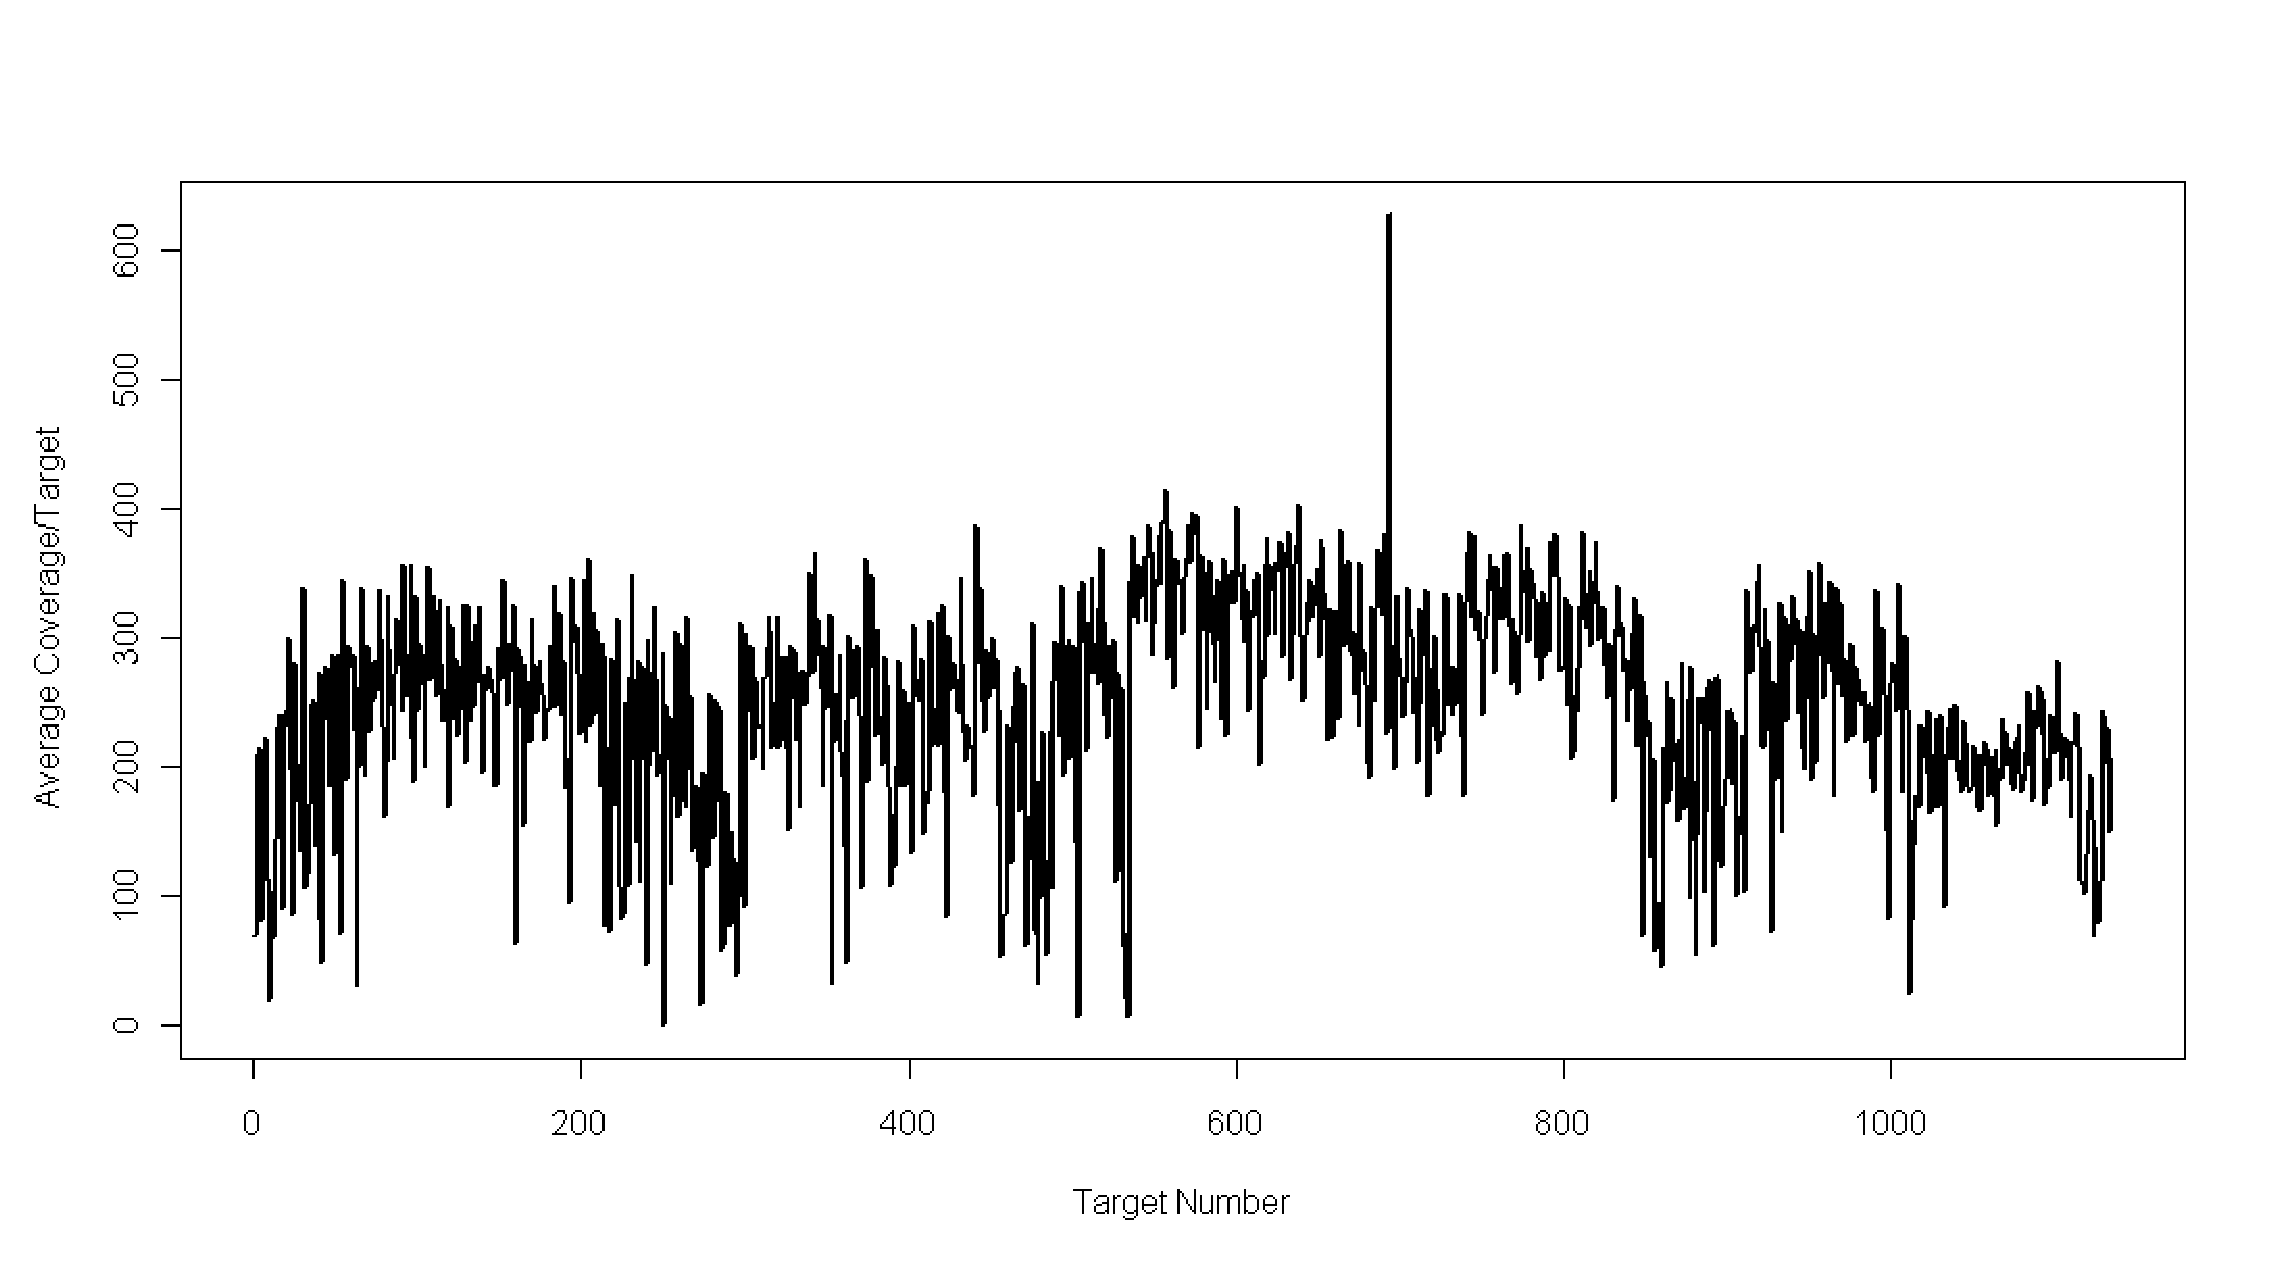
\includegraphics[width=1.0\linewidth]{img/SNP_Indel_Fig1}
	\caption[Average coverage per exon cardiomyopathy 48 gene panel]{Average coverage obtained from 22 different samples of all exon (1,133 exons) and exon/intron junctions ({$\pm$}20 bp) of 48 genes potentially involved in cardiomyopathy. 99\% of the targets show an average coverage of $\ge$30$\times$}.
	\label{fig:SNP_Indel_Fig1}
\end{figure}

\begin{figure}[!ht]
	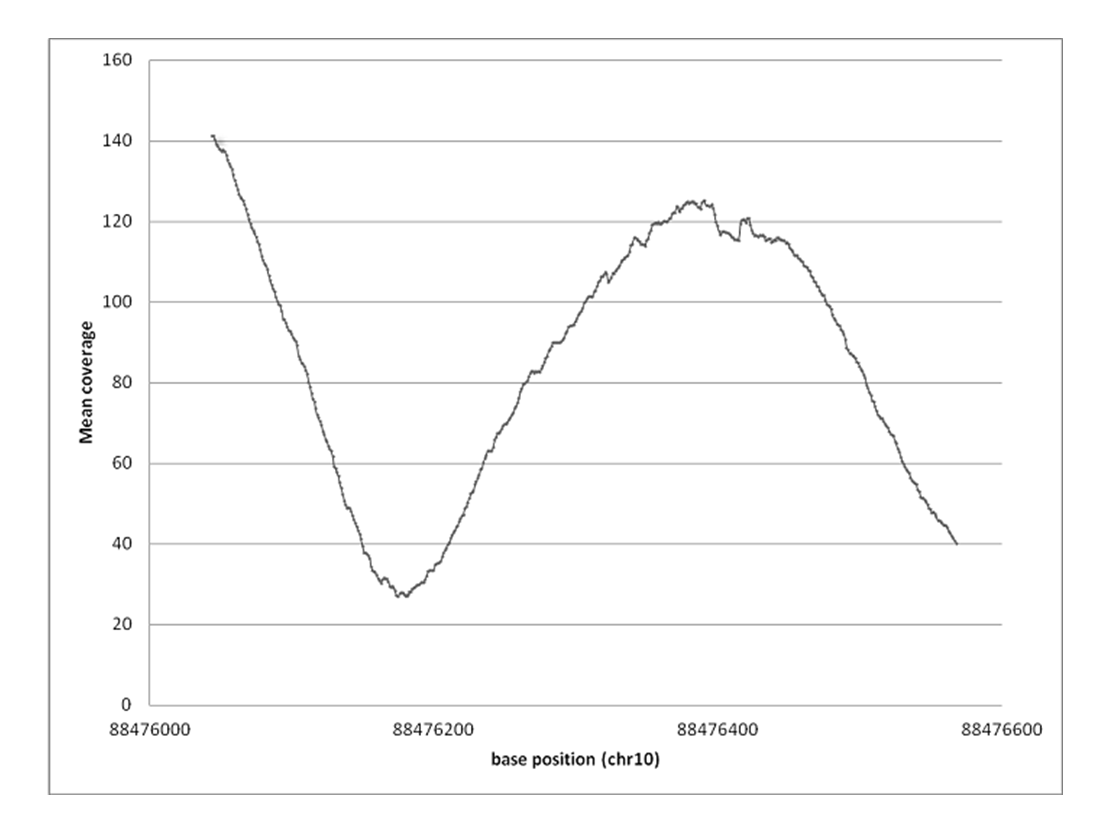
\includegraphics[width=1.0\linewidth]{img/SNP_Indel_Fig2}
	\caption[Coverage profile of single target \textit{LDB3} exon 9]{Coverage of one target, exon 9 of the \textit{LBD3} gene on chromosome 10 (NCBI build 37, UCSC hg19), representing one region with a coverage  $\le$30 in one patient.}
	\label{fig:SNP_Indel_Fig2}
\end{figure}


\begin{table}[!ht] %the []!ht] is to force the footnotes on the same page as the table
	\caption[Overview of the sequence performance for the validation runs]{\label{table:SNP_Indel_performance} Overview of the sequence performance for the validation runs}
	\tiny
	\resizebox{\linewidth}{!}{\begin{tabulary}{\linewidth}{p{3cm}p{2cm}p{2cm}p{2cm}}
			& Run 1 & Run 2 & Average of both runs \\
			\hline
			\rule{0pt}{1ex} Cluster density (k/mm\textsuperscript{2}) & 1,289 & 1,119 & 1,204  \\
			\rule{0pt}{1ex} \% Cluster PF & 89.3 & 94.6 & 92.0  \\
			\rule{0pt}{1ex} Q30 & 80.3 & 83.9 & 82.1  \\
			\rule{0pt}{1ex} Total reads & 17,168,243 & 15,788,049 & 16,478,146  \\
			\rule{0pt}{1ex} Matched reads & 16,414,062 & 15,186,556 & 15,800,309  \\
			\rule{0pt}{1ex} \% reads in .fasta file aligned & 96 & 96 & 96  \\
			\rule{0pt}{1ex} Mean mean coverage targets & 246 & 251 & 248  \\
			\rule{0pt}{1ex} Mean min coverage targets & 166 & 179 & 173  \\
			\rule{0pt}{1ex} Mean max coverage targets & 299 & 297 & 298  \\
			\rule{0pt}{1ex} \%Targets Mean {\textless}30 & 0.6 & 0.9 & 0.7  \\
			\rule{0pt}{1ex} \%Targets Mean {\textgreater}30 & 99.4 & 99.1 & 99.3  \\
			\rule{0pt}{1ex} \%Targets Min {\textless}30 & 2.6 & 2.5 & 2.6 \\
			\rule{0pt}{1ex} \%Targets Min {\textgreater}30 & 97.4 & 97.5 & 97.4  \\
			\rule{0pt}{1ex} \%Targets Max {\textless}30 & 0.4 & 0.7 & 0.5  \\
			\rule{0pt}{1ex} \%Targets Max {\textgreater}30 & 99.6 & 99.3 & 99.5  \\															
			\hline
	\end{tabulary}}
\end{table}


\subsubsection{Specificity and sensitivity of targeted NGS: confirmation of SS variants}
In previous SS analyses, a total of 90 variants in 14 different genes had been identified in the 24 patients used for validation (2 runs). 
All these variants were also detected with our targeted NGS approach applying the Agilent SureSelect kit (Fig. \ref{fig:SNP_Indel_Fig3}) and resulting in no false negatives. 
This included 84 substitutions and six indels (four deletions, two insertions). 
No additional variants were identified in these genes, comprising 55,784 bp. 
We therefore concluded that for these 24 samples there was full concordance with the SS results.

\begin{figure}[!ht]
	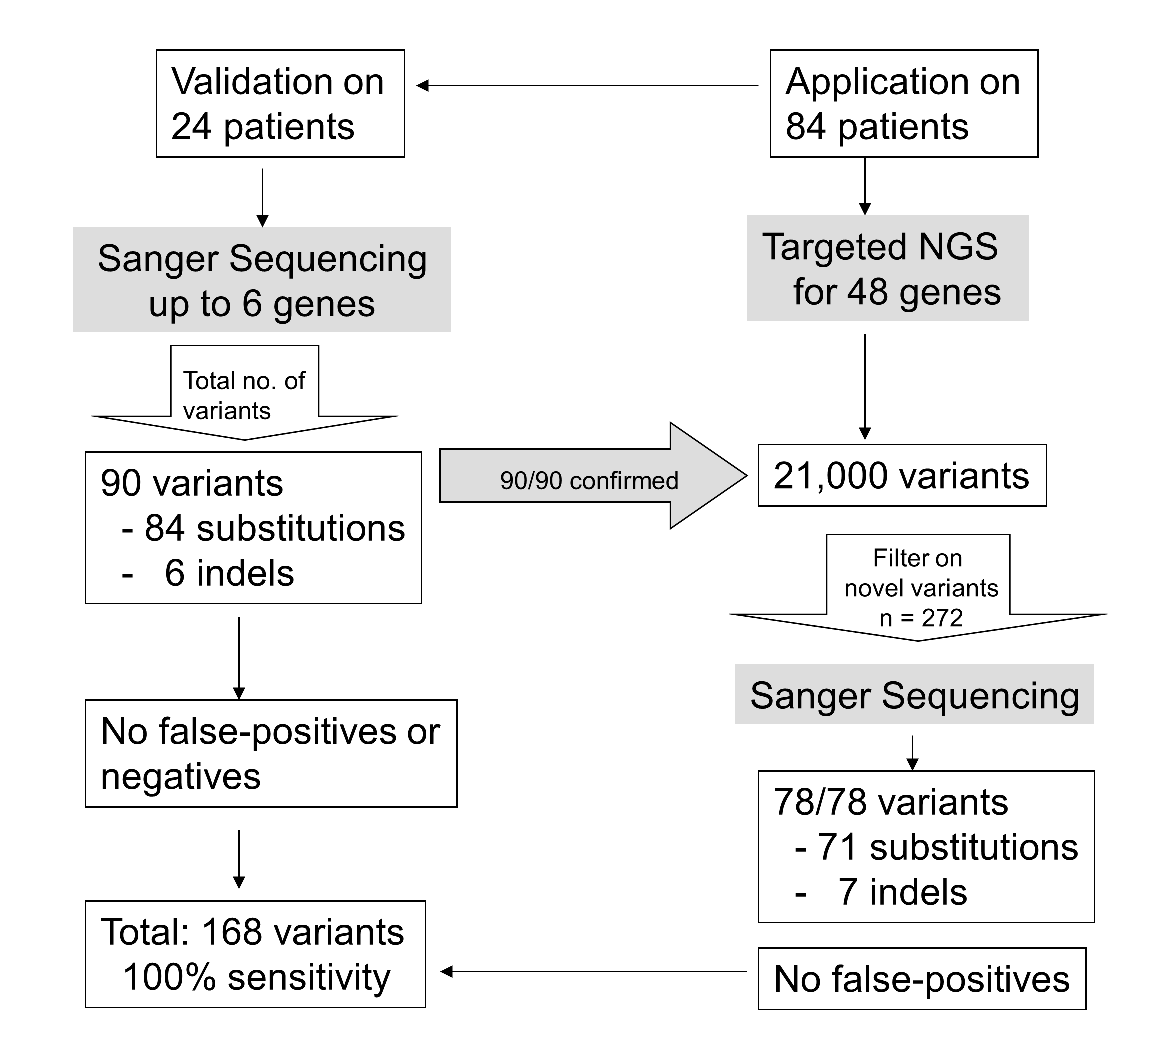
\includegraphics[width=1.0\linewidth]{img/SNP_Indel_Fig3}
	\caption[Summary of the results of our confirmation analyses]{Summary of the results of our confirmation analyses.}
\label{fig:SNP_Indel_Fig3}
\end{figure}

\subsection{Application phase}

\subsubsection{Sequence specificity of targeted NGS: confirmation of NGS variants}
Using targeted NGS of 48 genes, approximately 21,000 variants were identified in 84 unique patients (Fig. \ref{fig:SNP_Indel_Fig3}), including the 90 variants that had been previously detected with SS. 
Of these variants, 272 were novel (245 substitutions, 27 indels). 
On average, we identified three novel variants per patient. 
For validation with SS, 78 out of the 272 novel variants were selected, including detected indels (n = 7). 
The largest deletion comprised 18 bp and the largest insertion 8 bp. 
Notably, of the 71 substitutions, one was initially not confirmed by SS. 
This could be explained by the presence of a SNP in the primer binding site of the forward primer. 
A subsequent SS experiment, in which an alternative set of primers was used, did confirm the presence of this variant. 

In summary, a total of 168 variants were confirmed with SS. 
Based on these data, we reached a 100\% sensitivity (at 95\% confidence 97.76\%–100\%) \cite{Waerden_1957} with the NGS targeted approach.

\subsubsection{Diagnostic yield}
Applying this targeted NGS strategy, our first results indicate that the diagnostic yield is significantly improved from 15\% to about 40\%,mostly for DCM. 
However, this is based on small numbers of samples and the increase in yield may be even higher if this strategy is applied on a regular basis for larger series. 
Where regular routine diagnostics involves stepwise testing of up to about 10 different genes (which can easily take more than 1 year to complete), using targeted NGS of entire gene-panels on the MiSeq sequencer could theoretically provide reporting times of no more than 2 weeks. 
At this stage, we are aiming for reporting times of 4–6 weeks, a huge improvement compared with current diagnostic services.

\subsection{Reproducibility of targeted NGS}
The entire procedure was performed twice for five samples, including sequencing in different runs. 
On average, 231 variants (198–268) were detected per sample, and on average, 10 unique variants (8–14) were differently reported between the two analyses of identical samples. 
In total, 1,007 variants were detected and 51 of these were differently reported in the two separate analyses of the same sample resulting in a nonconcordance rate of 0.00315\% according to the number of sequenced bp (five times 323,651 bp of the targeted NGS kit). 
These differences can be attributed to three underlying causes: (1) in 12 out of 51 cases this was due to coverage differences, which meant variants were either not reported because of a too low coverage or reported when the coverage was just above threshold levels using the default settings; (2) in 24 out of 51 cases this was explained by alignment problems due to poly-T/A stretches, resulting in different annotating of the same variant; and (3) 15 out of 51 were due to differences in heterozygote levels, which meant variants that were present in {\textless}20\% of reads were not reported. 
Variants that fall within the first two categories are “true variants” that were either missed or reported as the result of analysis software settings or limitations. 
In contrast, variants in the third category most likely represent recurring technical artefacts, as all were repeatedly reported in a significant number of patients and in different runs, but were nonetheless not reported in the dbSNP and/or 1000 Genomes databases. 
Considering the artefacts as potential false positives the technical specificity is 0.0009269\%. 
In our future bioinformatic analyses, we will filter for the variants of the third category during our selection for potentially interesting variants, in addition to other filtering steps.

\section{Discussion}\label{discussion}
We present the validation of a targeted resequencing method for cardiomyopathy-associated genes and our results support its implementation in routine diagnostics. 
In this study, all the 168 variants identified by our NGS-approach were confirmed with SS (Fig.  \ref{fig:SNP_Indel_Fig3}). 
The variants included deletions up to 18 bp and insertions up to 8 bp. 
No false-negative or false-positive results were obtained for variants selected for confirmation. 
We therefore conclude that, at a coverage of at least 30 times per nucleotide, the performance of our procedure is comparable with SS. 

ES is likely to become the most commonly used tool for identifying genes in Mendelian diseases in the coming years \cite{Gilissen_2012}.
This approach has been shown to be successful in cases of rare monogenetic disorders \cite{Gilissen_2010,Hoischen_2010,Ng_2010} and of intellectual disability \cite{Vissers_2010}. 
However, as demonstrated by Gilissen et al. (2012)\cite{Gilissen_2012}, 2128 (5.7\%) of 37,424 disease-causing variant positions from the Human Genome Mutation Database are not covered with the 50Mb SureSelect ES kit (Agilent Technologies, Inc.). 
From our experience, we know that all the 48 genes we targeted are covered by probes in the 50Mb ES kit. 
However, the coverage performance varied significantly between exons within a gene and between different genes, and for some regions the coverage was {\textless}20 times, too low for reliable variant detection. 
This is exemplified by the \textsl{TTN} gene. 
Recently, Herman et al. (2012)\cite{Herman_2012} showed that \textsl{TTN} truncating mutations are a common cause of DCM, occurring in approximately 25\% of familial cases of idiopathic DCM and in 18\% of sporadic cases. 
From our ES data, we have calculated the average coverage per target for the coding regions of \textsl{TTN}. 
We found that 7\% of the targets sequenced had an average coverage of $\le$20 times (around 25 exons) and among those, 12 exons showed an average coverage of $\le$10 times. 
It is therefore very likely we would miss clinically relevant variants in these regions of low coverage. 
In contrast, the targeted region of the \textsl{TTN} gene in our designed kit shows a 100\% coverage for all exons and the respective nucleotides were all covered $\ge$30 times, with a high reproducibility between different samples. 
We therefore decided to continue developing our targeted resequencing method to overcome the shortcomings of incomplete representation and coverage of exons in ES experiments. 

The first prerequisite for high sensitivity of a NGS method is the development of a well-designed enrichment kit. 
We chose to use the SureSelect kit (Agilent Technologies, Inc.) as the e-Array programme used for kit design offered flexibility in optimizing the respective probe design. 
The number of tilings of each target can be chosen and extra baits can be added for GC-rich targets to increase coverage. 
A theoretical 100\% representation was reached for all of our targets. 
Based on our data, the theoretical representation given by e-Array is indicative for the actual coverage. 
Because the cost of a targeted custom-made enrichment kit is rather high, a good prediction of the coverage is an advantage before ordering such a kit for diagnostic use. 

The second prerequisite is high coverage of preferably all the targets. 
Setting the threshold at a coverage $\ge$30, we found only 50 targets out of the 1,134 with less coverage of the nucleotides, mostly in a part of the respective targets. 
We therefore decided that, parallel to targeted NGS, we will perform SS for targets with a low coverage from those genes of which the clinical relevance is uncontested (e.g., \textsl{MYH7}, \textsl{TNNI3} or \textsl{MYBPC3} for HCM; \textsl{LMNA}, \textsl{MYH7} or \textsl{MYBPC3} for DCM; and \textsl{PKP2} for ARVC) to ensure complete coverage of the respective amplicons (see Table \ref{table:SNP_Indel_recommendations} for general recommendations). 

\begin{table}[!ht] %the []!ht] is to force the footnotes on the same page as the table
	\caption[Diagnostic workflow and implementation guidelines]{\label{table:SNP_Indel_recommendations} Resulting diagnostic workflow and implementation guidelines}
	\tiny
	\resizebox{\linewidth}{!}{\begin{tabulary}{\linewidth}{p{3cm}p{6cm}}
			Workflow & Recommendations  \\
			\hline
			\rule{0pt}{1ex}  & \\
			\rule{0pt}{1ex} Enrichtment kit construction & Theoretically 100\% horizontal and vertical coverage of all targets  \\
			\rule{0pt}{1ex} Sample preparation &  \\
			\rule{0pt}{1ex} Days 1-3 & Automated, that is, using a Bravo or Caliper robot (Agilent Technologies, Inc./Caliper Life Sciences, Hopkinton, MA)  \\
			\rule{0pt}{1ex} Sample Enrichment & Bar-coding samples to a theoretical mean coverage of 250 for all targets resulting in a coverage of at least 30 per nucleotide in 98\% of targets  \\
			\rule{0pt}{1ex} Days 4-6 & Avoiding sample-mix-up by spiking unique DNA sequences before the procedure or including a limited SNP analysis for each individual patient  \\
			\rule{0pt}{1ex} Sequencing on bench-top machine & 80\% of the reads with Q30  \\
			\rule{0pt}{1ex} Days 7-8 &  \\
			\rule{0pt}{1ex} Data analysis & \\
			\rule{0pt}{1ex} Days 8-10 & Minimal coverage of 30 per nucleotide   \\
			\rule{0pt}{1ex}  & In house (control) variant database for filtering \\
			\rule{0pt}{1ex}  & A predifined variant filtering procedure, preferably automated in software programmes like the NGS bench lab from CARTAGENIA (Leuven, Belgium)  \\
			\rule{0pt}{1ex} Confirmation with Sanger Sequencing &  \\
			\rule{0pt}{1ex} Days 11-20 & Obsolete at a coverage of {\textgreater}30 per nucleotide \\
			\rule{0pt}{1ex}  & Coverage of targets structurally below 20: Sanger sequencing in parallel with NGS \\
			\rule{0pt}{1ex}  & Incidental coverage below 20: Sanger sequencing depending on the target's clinical relevance \\
			\rule{0pt}{1ex}  & Coverage between 20 and 30: visual inspection, Sanger sequencing of novel variants  \\
			\rule{0pt}{1ex} Total turn-around time & 21 days  \\															
			\hline
	\end{tabulary}}
\end{table}
\addtocounter{footnote}{1}
\footnotetext{ Basepair position according to NCBI build 37}

\noindent Valencia et al. (2012)\cite{Valencia_2012} developed a SureSelect enrichment kit for congenital muscular dystrophy for 321 targets (12 genes) and 95\% of them had a coverage of at least 20. 
According to their data, the coverage was below 20 times for two genes due to a high GC content. 
In contrast, our kit represents a much better coverage (99\% covered more than 30 times). 
There are several explanations for this difference, for instance the tiling of the baits, differences in the overall GC content, or the number of pooled patients, which make a good comparison difficult. 
In our approach, 12 samples were pooled based on the size of the enrichment kit to reach a coverage of at least 30 times per basepair for most of the targets. 
Because no false-positive or -negative results were detected, this would seem to be a safe threshold. One could even consider whether more than 12 patients could be pooled or the coverage threshold reduced to {\textgreater}20 times instead of {\textgreater}30 times. 
In Table \ref{table:SNP_Indel_recommendations}, we give some general recommendations on the clinical laboratory implementation and quality assessment of targeted resequencing methods. 
These recommendations are in line with the general guidelines for assuring the quality of NGS in clinical laboratory practice formulated by the national workgroup of the US Centers for Disease Control and Prevention \cite{Gargis_2012}.

A 100\% sensitivity (95\% confidence: 97.76\%–100\%) was reached with our approach and a specificity of nearly 100\% (0.00315\% false positive). 
Gowrisankar et al. \cite{Gowrisankar_2010} reported a false-positive rate of 0.011 $\pm$ 0.002\%, close to 100\% specificity for 41,475 bp using an Illumina GAII sequencing machine and targeted resequencing of 19 DCM genes. 
However, four out of the 160 basepair substitutions and three out of 31 indels were missed, including one 18 bp duplication. 
The basepair substitutions were missed because of insufficient coverage ({\textless}30 times), whereas the indels were likely missed due to sequencing of short read lengths (36 bp). 
In our approach, 151 bp reads were used and we were able to detect an 18 bp deletion, the largest indel detected in our study. 
In total, 17 indels detected were confirmed with SS, but it is debatable how many and which type of indels should be confirmed by SS for proper validation. 
Depending on the gene panel to be sequenced, it seems obvious to choose patients with the largest known indels for validation. 
Gowrisankar et al. \cite{Gowrisankar_2010} recently reported an 18 bp duplication and Herman et al. \cite{Herman_2012} a 13 bp deletion in the \textsl{titin} gene, which seem to be the largest indels associated with cardiomyopathies so far. 
As indels of that size were detected in our procedure, we are convinced we can retain 100\% sensitivity. 
Moreover, according to our results, we would have missed one variant with SS due to a SNP in the primer sequence. 
This suggests that resequencing after hybridization-based enrichment of targets may even outperform SS. 

The importance of longer read lengths was underscored by the results of Voelkerding et al. \cite{Voelkerding_2010}. 
They performed SureSelect enrichment for 12 genes responsible for congenital muscular dystrophy in combination with sequencing on a SOLiD machine. 
Two out of the 34 identified variants were not confirmed with SS because of sequence read misalignment between two closely related genes. 
As a probe based method, not only targeted sequences but also highly homologous pseudogenes and other homologous sequences, such as those present in gene families and domain analogs will be captured \cite{Coonrod_2012}. 
Highly homologous sequences coalign to the reference sequence. 
However, it is uncertain to what extent regions of high-homology may negatively affect the sensitivity and specificity. 
In general, construction of a unique tiled bait library using differences in the neighboring intron sequences and eventually longer paired end reads can reduce this problem. 

The reproducibility of our procedure was tested by repeating the procedure for five samples. 
The 99.99685\% concordance of all detected variants demonstrates the high performance of our targeted enrichment and MiSeq resequencing method. 
Apart from low coverage an alignment problem due to poly A/T stretches resulted in discrepancies. 
However, these variants will not result in false positives. 
Discrepancies due to differences in the heterozygote level of 20\% might be considered as technical false positives (0.0009269\%). 
However, according to our analyses criteria we would have filtered these variants out. 
In summary, the differences seen between the separate analyses of the five repeated samples were due to bioinformatic threshold and annotation settings and not due to technical limitations. 
Variants with an allelic imbalance need careful follow up. 
This is in line with the first report on a MiSeq-based sequencing method in which drafting genomic sequences of \textsl{E. coli} resulted in an error rate of 0.1 substitutions per 100 bases and a near absence of indel errors \cite{Loman_2012}. 
This, together with the almost 100\% sensitivity and specificity of our results, raises the question whether a variant still needs to be confirmed with SS, as is often daily practice in clinical diagnostics at the moment. Zhang et al. \cite{Zhang_2012} felt it was necessary for two reasons: first, to remove incorrect calls due to experimental errors, and second, to confirm a diagnosis. 
However, as they discussed, confirmation becomes burdensome or impossible when a large number of novel variants need to be confirmed and this would result in long turn-around times. 
We therefore propose to refrain from confirming results with SS as long as the coverage is {\textgreater}30 times per nucleotide. 
In addition, targets that are not covered or badly covered can either be excluded from the final report or SS of these targets can be performed in parallel. 
At a coverage between 30 and 20 times, visual inspection of the regions is recommended (see Table \ref{table:SNP_Indel_recommendations} for general recommendations).

\section{Conclusion}
Our data convincingly demonstrate that targeted NGS of a disease-specific subset of genes can be reliably implemented as a stand-alone diagnostic test.

\section{Acknowledgments}\label{Acknowledgments} 
We thank Jackie Senior for editorial advice.


\subsubsection{Disclosure Statement} 
The authors declare no conflict of interest.

